% \documentclass[twocolumn]{article}
\documentclass{article}
% \documentclass[useAMS,usenatbib]{mnras}
\usepackage[utf8]{inputenc}

\usepackage{graphicx}% Include figure files
\usepackage{xcolor}
\usepackage{epstopdf}% Allows eps figures
\usepackage{float}% Better image placement
\usepackage{enumerate}

\usepackage{textcomp,gensymb}% Adds general symbols
\usepackage{amsmath, amssymb}% Math symbols and stuff
\usepackage{mathtools}% math things

\usepackage[numbers,sort&compress]{natbib}% Hyperlink References
\usepackage{hyperref}% Hyperlink References

\usepackage{ulem}
\usepackage[capitalise]{cleveref}

\newcommand{\dnp}[1]{\textcolor{cyan}{#1}}


\title{Quick Notes about Machine Learning on Intensity Maps}
\author{Daniel N. Pfeffer}
\date{}

\graphicspath{{images/}}

\begin{document}
% \bibliographystyle{unsrtnat}

	\maketitle

	\begin{abstract}
		The idea of this project is to use machine learning on intensity maps to determine the luminosity function of the underlying halos.
	\end{abstract}

	\section{Intensity Maps Background} \label{sec:IMback}

		Intensity mapping is done by looking at a given emission line.  Whatever is being traced should be emitting this line at any location where the tracer is located.  Having a higher density of the tracer would cause an increased intensity of whatever line is being looked at.  As the light travels to Earth it will get redshifted based on where it was originally emitted.  By looking at a range of frequencies one can get 3D spatial information (maps) about whatever tracer is being looked at.  

		George has code to generate different halo catalogs quickly and has done so to make (as of the time of writing this part) 161 halo catalogs.  Each of these catalogs can be converted into smaller subfields as well as rotated to produce more catalogs.  With another code of George's one can convert these halo catalogs (or regions in them) into intensity maps.  We want lots of intensity maps so that we can do machine learning on the maps to determine the underlying luminosity function.

	\section{Machine Learning Background} \label{sec:MLback}

		I'm feeling lazy right now and don't want to fully flesh this out yet.

		Machine learning can be used for lots of tings if you throw enough data at it.  

		Neural networks are supposed to represent how brains and neurons work.  It is trained for a specific task and each neuron has it's own weights.  This gets very memory intensive for large networks because there can be lots of neurons.  A way around this is to use convolutional neural networks (CNN).  A CNN has filters that convolve with layers of input or neuron output and each layer has the same filter which saves on memory.  A quick Google showed these links that explain CNNs both in depth (http://cs231n.github.io/convolutional-networks/) and at a surface level (https://medium.freecodecamp.org/an-intuitive-guide-to-convolutional-neural-networks-260c2de0a050).

	\section{Intensity Mapping CNN (Actually on N not dN/dL)} \label{sec:cnn}

		As of right now the idea is to use a CNN on simulated intensity maps to determine the luminosity function of the underlying halos that made the simulated intensity maps.  George has code to make the halo catalogs and another code to convert the catalogs into intensity maps.  I've made code to split up the catalogs into smaller subfields to match possible experiments.  I also have code that will rotate the halo catalogs before making subfields so that we have more subfields to train out network with.  George's code limlam mocker (llm) (the code that converts catalogs into intensity maps) was modified by me to also give out the luminosity function of the underlying halos.  The llm can also use different underlying halo luminosity relations to generate different maps and luminosity functions.

		As of the basic training right now I am not doing anything to split up the maps into training, validation and test sets.  I'm just seeing the general results of different things right now.

		\subsection{log dN/dL} \label{sec:logValue}
			Originally the CNN was trained on converting an intensity map into \(\log dN/dL\) instead of just \(dN/dL\).  This was done originally to prevent having such a large range of output values could be hard to train.

			As of right now I have a trained network that is 4 layers that trained for 100 epochs of 400 maps apiece.  Each layer is a 3D convolution with kernel size 5 and stride 1 followed by a max pooling 3D of size 2 and stride 2.  The first layer has 32 filters, followed by 64, 128 and 256.  Following the convolutional layers the network is flattened and then has a dense layer with 1000 neurons.  The final layer is another dense layer with a neuron for each point in the luminosity function we want.  Currently I take 50 points of the luminosity function.  The loss function was just the mean square error function.

			\dnp{Should get plots for accuracy and loss as a function of time, but forgot to add that functionality to the CNN when I first ran it}.  The network took under 30 hours to train.  \cref{fig:CNN_4_layer_log,fig:CNN_4_layer_log_ratio,fig:CNN_4_layer_log_ratio_small} show the result of the CNN on some random map.  In all luminosity bins before around \(L = 10^6 L_{sun}\) the CNN luminosity function is within a couple of percent of the underlying one.  After \(L = 10^6 L_{sun}\) the ratio of CNN luminosity function to the given luminosity function jumps up to around 1.6.  The specific values change depending on what map is used, but they all show the issue at large luminosities.

			\begin{figure}[H]
				\centering 
				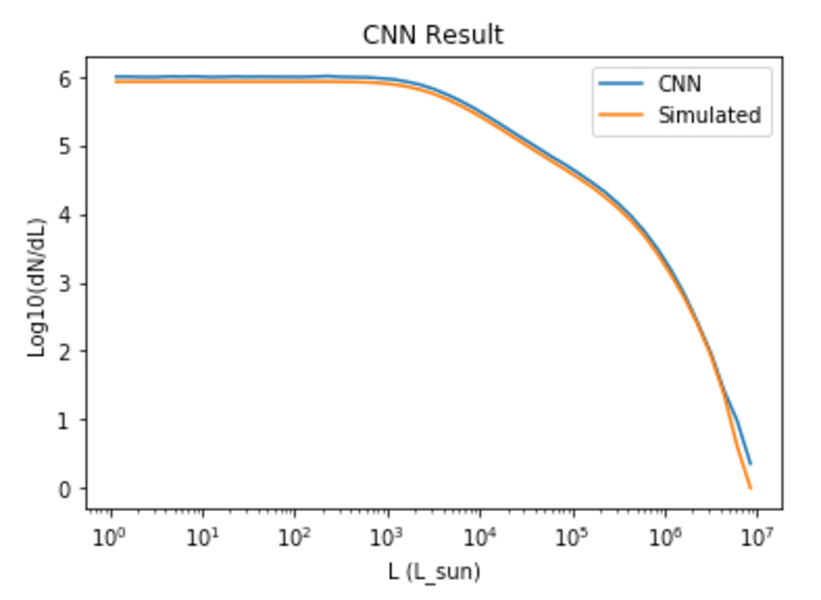
\includegraphics[width=0.8\textwidth]{CNN_4_layer_log.pdf}
				\caption{Plot showing the comparison of the output of the 4 layer CNN to the expected result of the underlying luminosity function that made the intensity map.}
				\label{fig:CNN_4_layer_log}
			\end{figure}

			\begin{figure}[H]
				\centering
				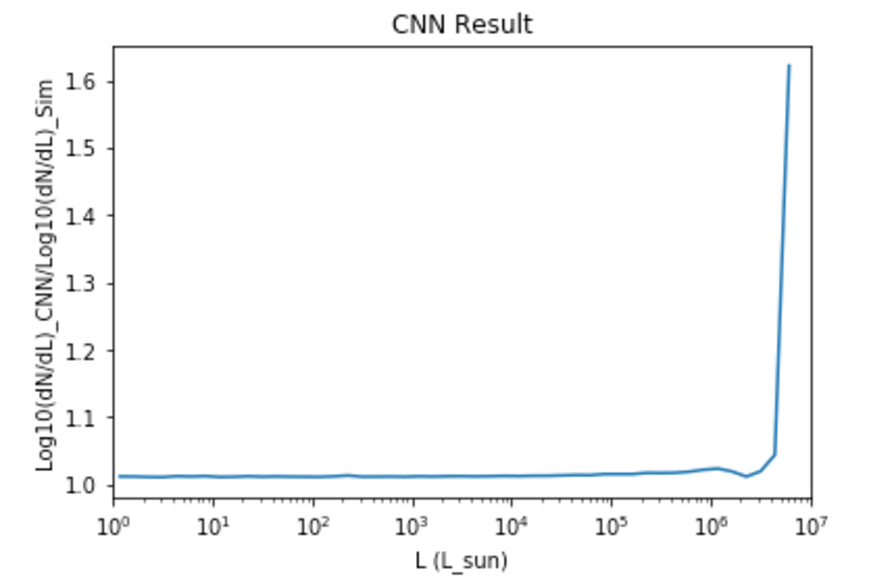
\includegraphics[width=0.8\textwidth]{CNN_4_layer_log_ratio.pdf}
				\caption{Plot showing the ratio of the CNN luminosity function over the underlying luminosity function.}
				\label{fig:CNN_4_layer_log_ratio}
			\end{figure}

			\begin{figure}[H]
				\centering
				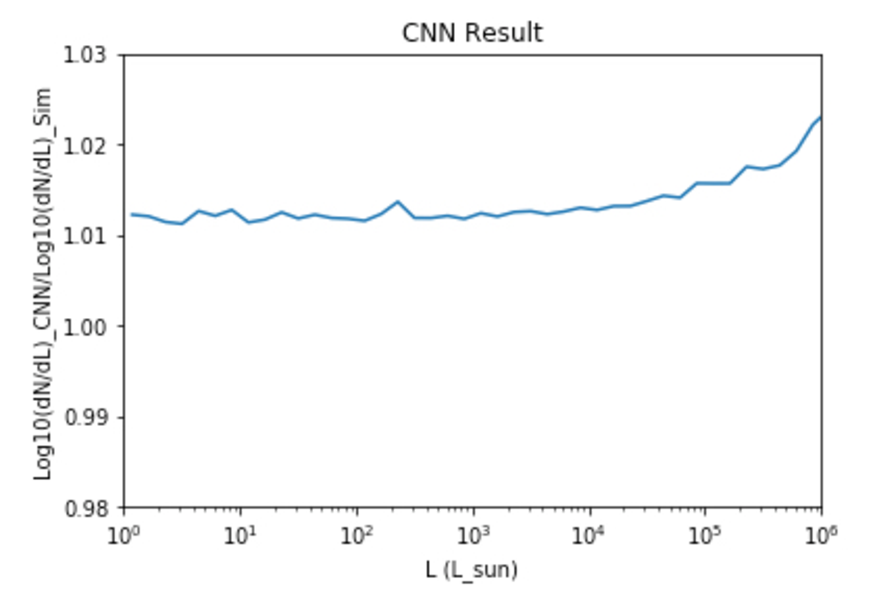
\includegraphics[width=0.8\textwidth]{CNN_4_layer_log_ratio_small.pdf}
				\caption{Zoom in of Figure \ref{fig:CNN_4_layer_log_ratio} showing the ratio of values before \(L = 10^6 L_{sun}\).}
				\label{fig:CNN_4_layer_log_ratio_small}
			\end{figure}

			We are probably interested in the actual values of things and not the log value so I checked the accuracy of the values instead of the log values.  The same set of plots but without logs are shown in \cref{fig:CNN_4_layer_log_unlog,fig:CNN_4_layer_log_unlog_ratio,fig:CNN_4_layer_log_unlog_ratio_small}.  What can be seen is that the error increases by at least an order of magnitude.  The error is still only around 20\%, but is still much larger then in the log case.  It can be shown (but I'm too lazy to type it out now) that the ratio of the unloged values is actually given by
			\begin{equation}
				\frac{dN}{dL}_{\rm{CNN}} / \frac{dN}{dL}_{\rm{sim}}(L) = 10^{\log \left(\frac{dN}{dL}_{\rm{sim}} (L)\right) * y(L)}
			\end{equation}
			where 
			\begin{equation}
				y = \log \left( \frac{dN}{dL}_{\rm{CNN}} \right) / \log \left( \frac{dN}{dL}_{\rm{sim}} \right)(L).
			\end{equation}

			\begin{figure}[H]
				\centering
				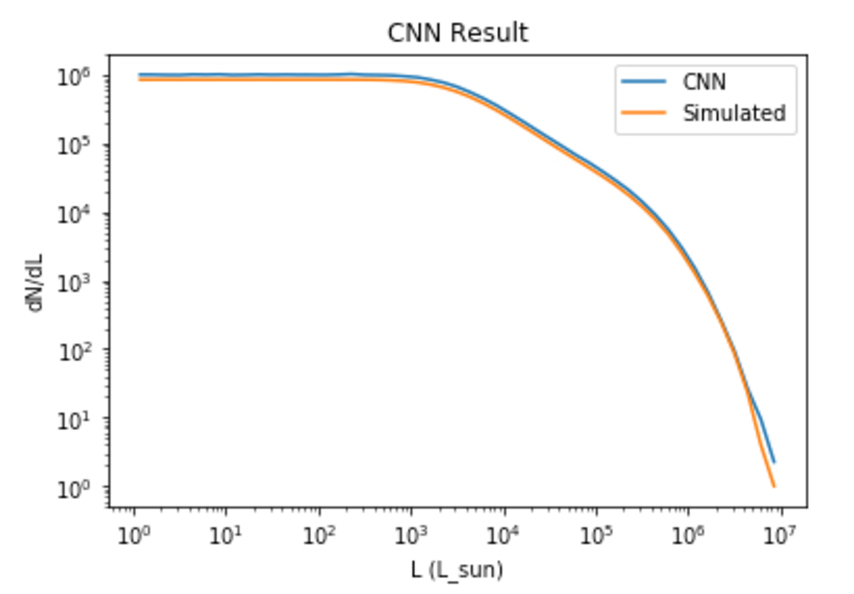
\includegraphics[width=0.8\textwidth]{CNN_4_layer_log_unlog.pdf}
				\caption{Plot showing the comparison of the output of the 4 layer CNN to the expected result of the underlying luminosity function that made the intensity map.}
				\label{fig:CNN_4_layer_log_unlog}
			\end{figure}

			\begin{figure}[H]
				\centering
				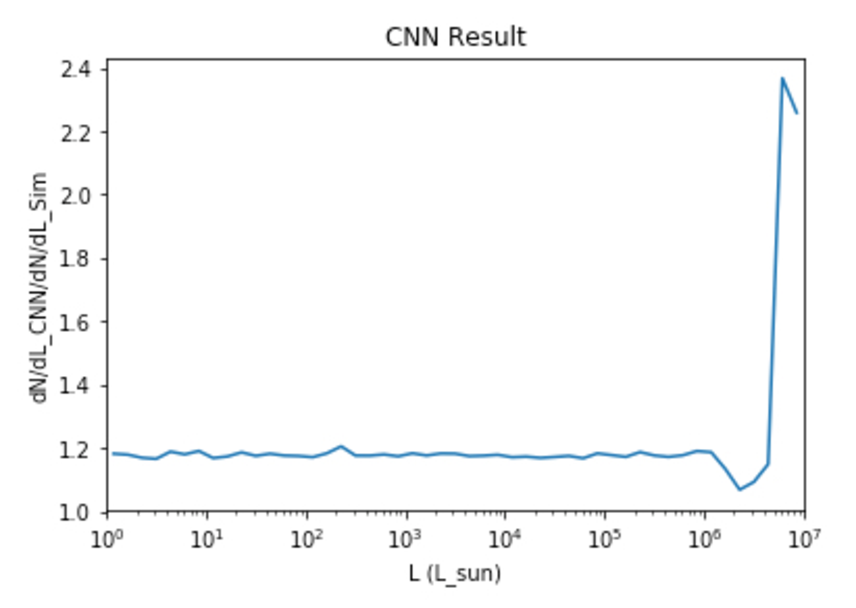
\includegraphics[width=0.8\textwidth]{CNN_4_layer_log_unlog_ratio.pdf}
				\caption{Plot showing the ratio of the CNN luminosity function over the underlying luminosity function.}
				\label{fig:CNN_4_layer_log_unlog_ratio}
			\end{figure}

			\begin{figure}[H]
				\centering
				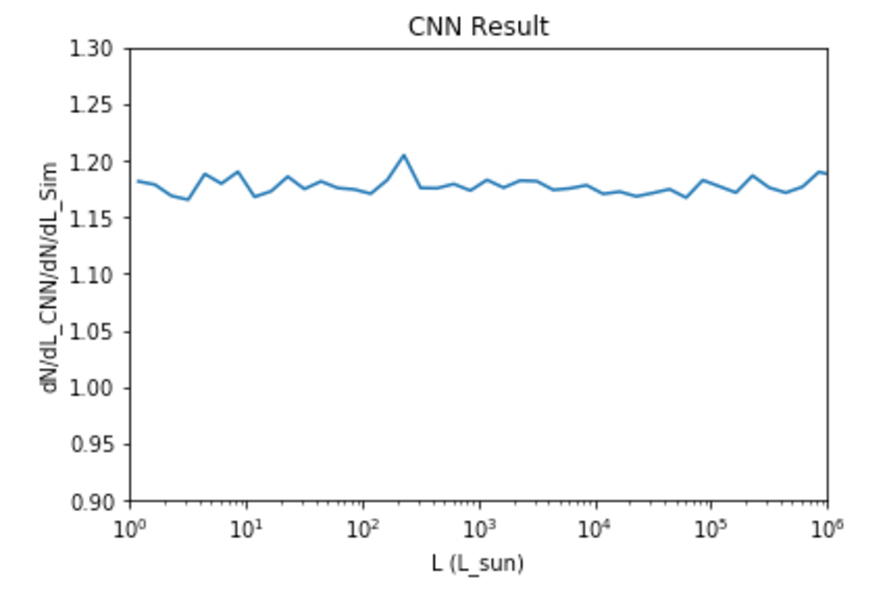
\includegraphics[width=0.8\textwidth]{CNN_4_layer_log_unlog_ratio_small.pdf}
				\caption{Zoom in of Figure \ref{fig:CNN_4_layer_log_ratio} showing the ratio of values before \(L = 10^6 L_{sun}\).}
				\label{fig:CNN_4_layer_log_unlog_ratio_small}
			\end{figure}

		\subsection{4 Layer dN/dL} \label{sec:4directValue}
			Seeing that finding the log luminosity value gives errors around 20\%, I tried to see if we could find the actual luminosity function directly.  The first network was 4 layers and was trained for 100 epochs of 400 maps apiece.  Each layer is a 3D convolution with kernel size 5 and stride 1 followed by a max pooling 3D of size 2 and stride 2.  The first layer has 32 filters, followed by 64, 128, 256 512.  Following the convolutional layers the network is flattened and then has a dense layer with 1000 neurons.  The final layer is another dense layer with a neuron for each point in the luminosity function we want.  Currently I take 50 points of the luminosity function.  The loss function was the mean log square error function.  Using mlse instead of mse makes it so that it doesn't get stuck trying to fit the region of low L and ignore the higher L regions where dN/dL is smaller. 

			I forget how long the network took to train, but it was under 48 hours.  Looking at \cref{fig:CNN_4_layer,fig:CNN_4_layer_ratio} one can see that the training did not go as well as it could.  There are discontinuities in the outputted luminosity function, sharp spikes and nothing after \(L \approx 10^6 L_{\rm{sun}}\).  I'm no expert, but we would want something better then that.  \cref{fig:CNN_4_layer_history_mlse,fig:CNN_4_layer_history_mse} show the training history of the loss function and another metric as a function of epoch while training 4 layer network.  The shape of \cref{fig:CNN_4_layer_history_mse} does look like what one would expect from a loss function.

			\begin{figure}[H]
				\centering
				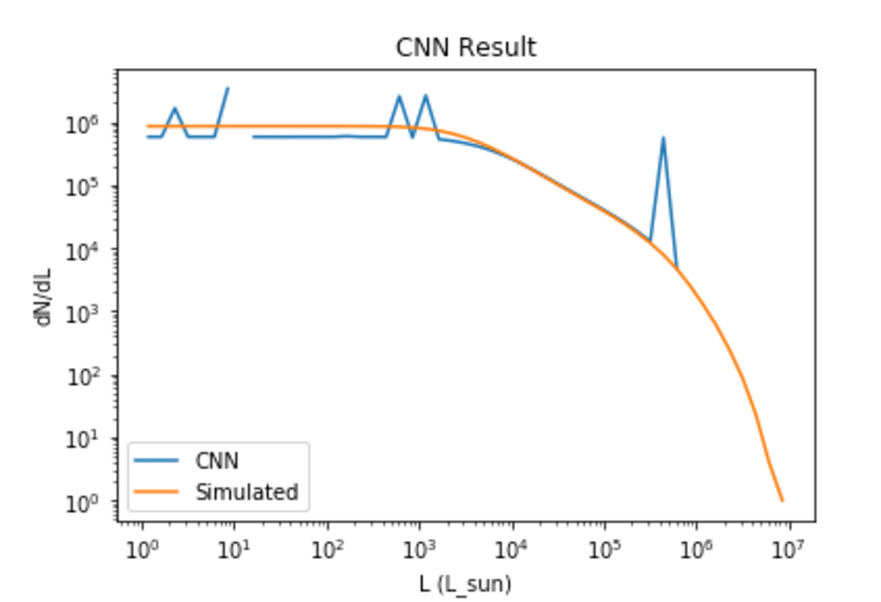
\includegraphics[width=0.8\textwidth]{CNN_4_layer.pdf}
				\caption{Plot showing the comparison of the output of the 4 layer CNN to the expected result of the underlying luminosity function that made the intensity map.}
				\label{fig:CNN_4_layer}
			\end{figure}

			\begin{figure}[H]
				\centering
				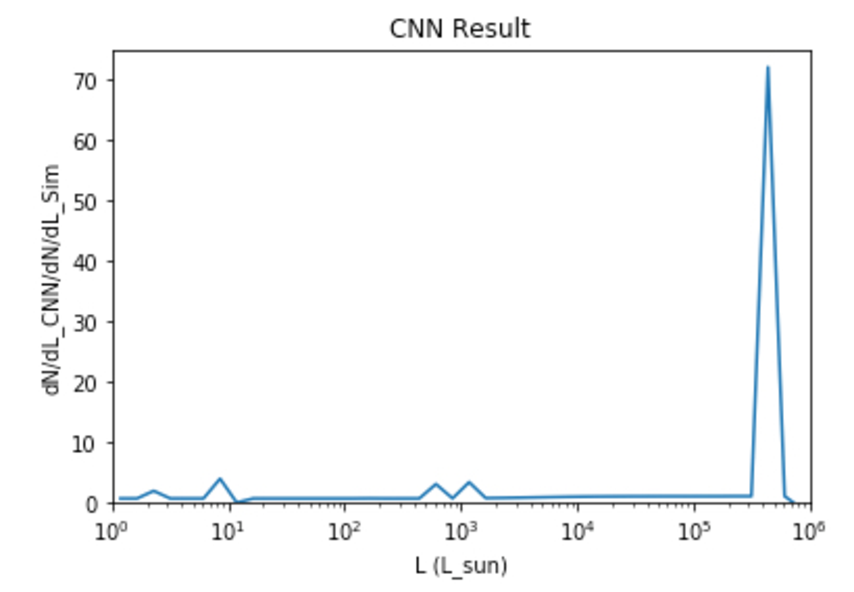
\includegraphics[width=0.8\textwidth]{CNN_4_layer_ratio.pdf}
				\caption{Plot showing the ratio of the CNN luminosity function over the underlying luminosity function.}
				\label{fig:CNN_4_layer_ratio}
			\end{figure}

			\begin{figure}[H]
				\centering
				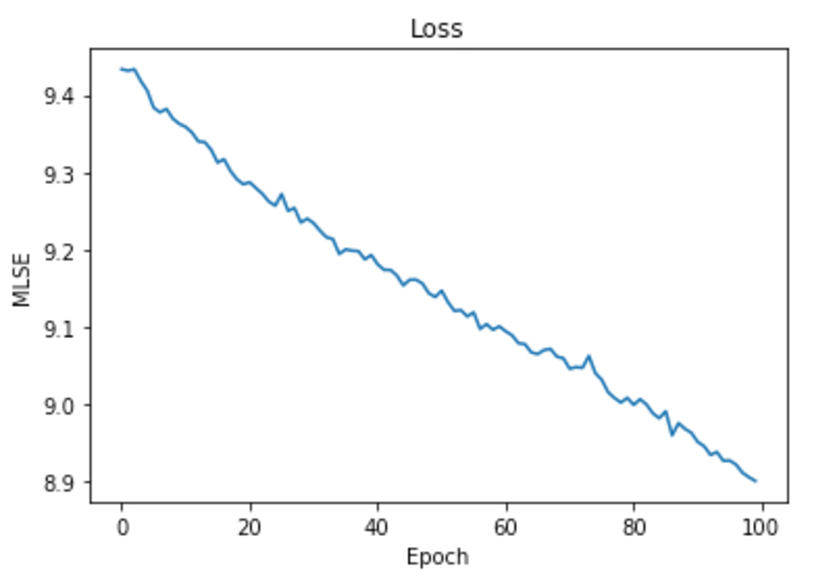
\includegraphics[width=0.8\textwidth]{CNN_4_layer_history_mlse.pdf}
				\caption{Plot showing loss history of the 4 layer CNN that was trained on the full luminosity function.  The loss function that was used was the mean log squared error}
				\label{fig:CNN_4_layer_history_mlse}
			\end{figure}

			\begin{figure}[H]
				\centering
				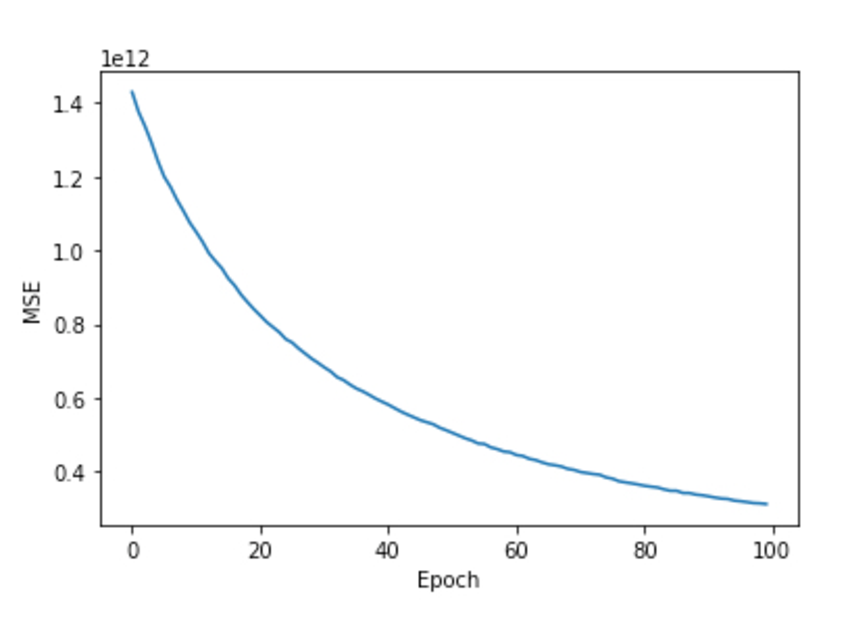
\includegraphics[width=0.8\textwidth]{CNN_4_layer_history_mse.pdf}
				\caption{Plot showing history of the mean squared error metric as a function of epoch.}
				\label{fig:CNN_4_layer_history_mse}
			\end{figure}

		\subsection{5 Layer dN/dL} \label{sec:5directValue}
			I tried making a 5 layer network, but it was much slower and only got around 30 epochs in 48 hours.  It was way too slow to train.  I saved every 20 epochs so not everything was wasted.  \cref{fig:CNN_5_layer} shows how "good" the semi-trained network is and it is pretty bad.  This needs more time.  I'm trying to run it for longer now and see if it will hopefully turn out better then the 4 layer network.

			\begin{figure}[H]
				\centering
				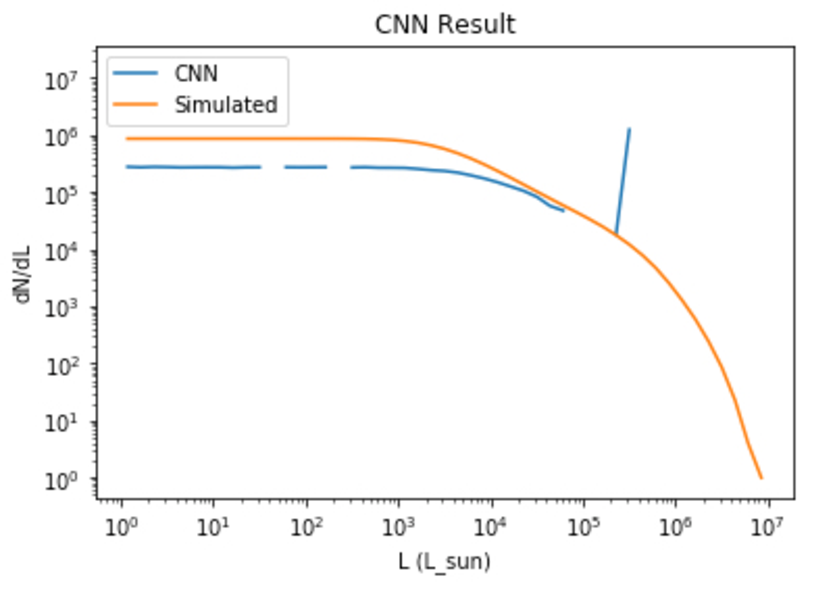
\includegraphics[width=0.8\textwidth]{CNN_5_layer.pdf}
				\caption{Plot showing the comparison of the output of the 5 layer CNN to the expected result of the underlying luminosity function that made the intensity map.}
				\label{fig:CNN_5_layer}
			\end{figure}

	\section{Intensity Mapping CNN (On dN/dL this time)} \label{sec:cnn2}
		The previous shown work was done using the number count instead of the luminosity function.
		\begin{equation}
			N = \int_{L_*}^{\inf} \phi dL
		\end{equation}
		Using the actual luminosity function instead of the number count gives worse results.  I believe this is due to the fact that instead of something that is monotonically decreasing we have to worry about more features.  I think if we converted this to a Fourier space analog and looked at power at different scale we would find more power at lower scales when looking at \(\phi\) rather then \(N\).  In \cref{fig:compare_N_to_phi} we see for a given map the difference between the normalized number counts and normalized luminosity function.  The luminosity function has more features.  These extra features require more training on the part of the CNN.  Training on number counts will be faster and produce better results then the luminosity function.

		\begin{figure}[H]
			\centering
			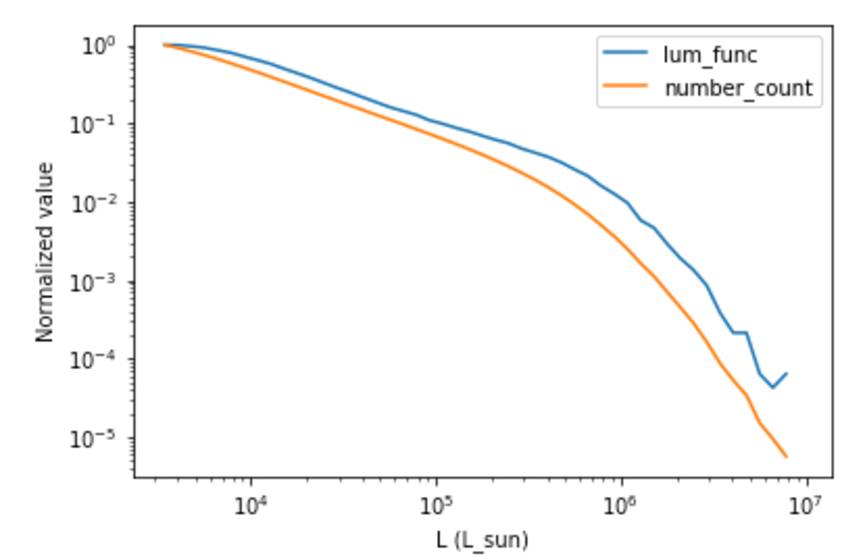
\includegraphics[width=0.8\textwidth]{compare_N_to_phi.pdf}
			\caption{Figure showing the differences between normalized \(N\) and \(\phi\).  The lum func line is \(\phi(L)\) and number count is \(N(L)\).  The main thing to notice is that there are more features in the \(\phi\) curve then the \(N\) curve.}
			\label{fig:compare_N_to_phi}
		\end{figure}

		While training models I get stupid errors that I don't really know every once and a while.  It is some stupid cuda error which makes it very hard to debug and I can't reproduce them.  Just going to throw one of them here so it is in the record.  Line breaks were added by me.

		\begin{verbatim}
			F tensorflow/stream_executor/cuda/cuda_dnn.cc:521] 
			Check failed: cudnnSetTensorNdDescriptor(handle_.get(), 
			elem_type, nd, dims.data(), strides.data()) == 
			CUDNN_STATUS_SUCCESS (3 vs. 0)
			batch_descriptor: {count: 0 feature_map_count: 16 
			spatial: 252 252 96  value_min: 0.000000 
			value_max: 0.000000 layout: BatchDepthYX}
		\end{verbatim} 

		There were also issues with trying to train on \(\phi L\).  I don't know what the network was doing, but it would just start getting nulls, nans or infs for output pretty quickly or it would just give garbage in the end.  It is probably something I'm doing, but maybe the architecture doesn't like the shape of \(\phi L\) as seen in \cref{fig:phi_L}.  it is more complicated then either \(N\) or \(\phi\).

		\begin{figure}[H]
			\centering
			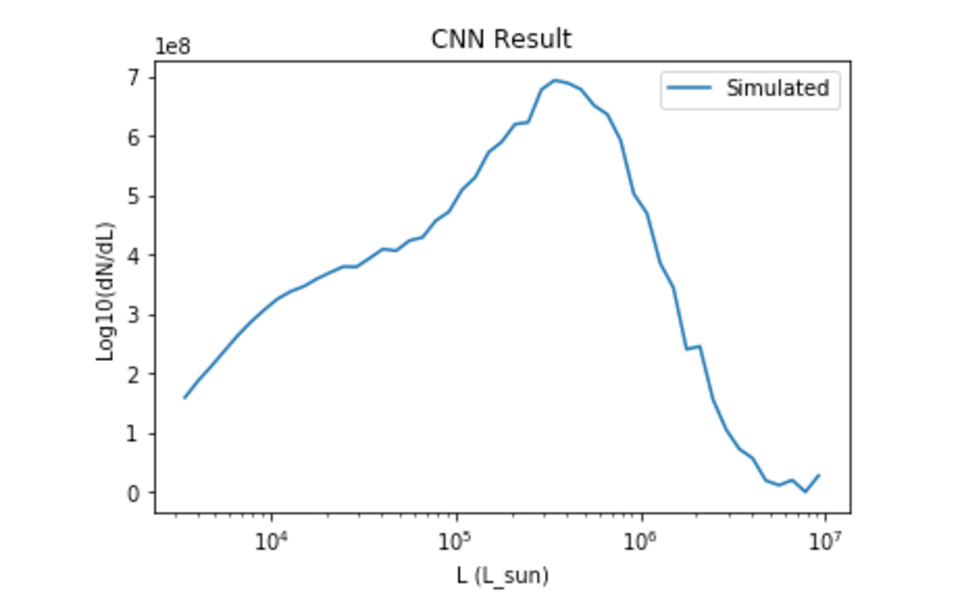
\includegraphics[width=0.8\textwidth]{phi_L.pdf}
			\caption{A generic look at what \(\phi L\) v.s. \(L\) should look like.}
			\label{fig:phi_L}
		\end{figure}

		\subsection{2D v.s. 3D}
			When designing the CNN we have a choice between doing 2D or 3D convolutions.  3D makes things much slower and requires more space.  A comparison between 2D and 3D models can be seen in \cref{fig:2d_vs_3d}.  From the figure it is clear that the 2D model beats the 3D one and the longer running 2D model does best.  The 3D model just doesn't look good.  I can't get it to actually work for the log values.  I don't have a model for 5 layers due to it failing at some point while running.

			\begin{figure}[H]
				\centering
				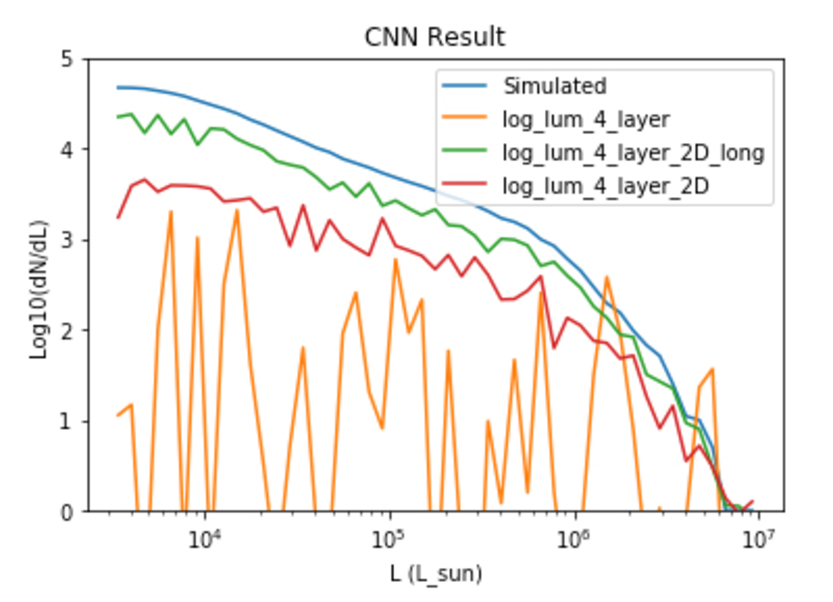
\includegraphics[width=0.8\textwidth]{2d_vs_3d.pdf}
				\caption{A comparison between three different models.  For two of them the difference between them was that one was with 3D convolutions and the other with 2D ones.  Their epochs were roughly the same number of evaluations and they had the same number of epochs.  The long model was run with more evaluations per epoch rather then more epochs.}
				\label{fig:2d_vs_3d}
			\end{figure}

			It seems, at least for the log values, that it is better to go with the 2D convolutions.  It is faster, more space efficient and gives better results.

			We can compare the loss history of the 2D and 3D models in \cref{fig:log_lum_4_layer_2D_history,fig:log_lum_4_layer_history} to try and see what's going on.  The history for the 3D one is garbage.  The validation loss never goes down.  I don't fully understand what is happening.  Naively this would mean that it is memorizing the training data and not knowing the validation data.  The issue with this is that if I run the model on data that should have been training data it still returns garbage.  The 2D model is better.  The validation data does improve, but it stalls out around halfway through and doesn't improve much anymore.  It does show learning though.

			\begin{figure}[H]
				\centering
				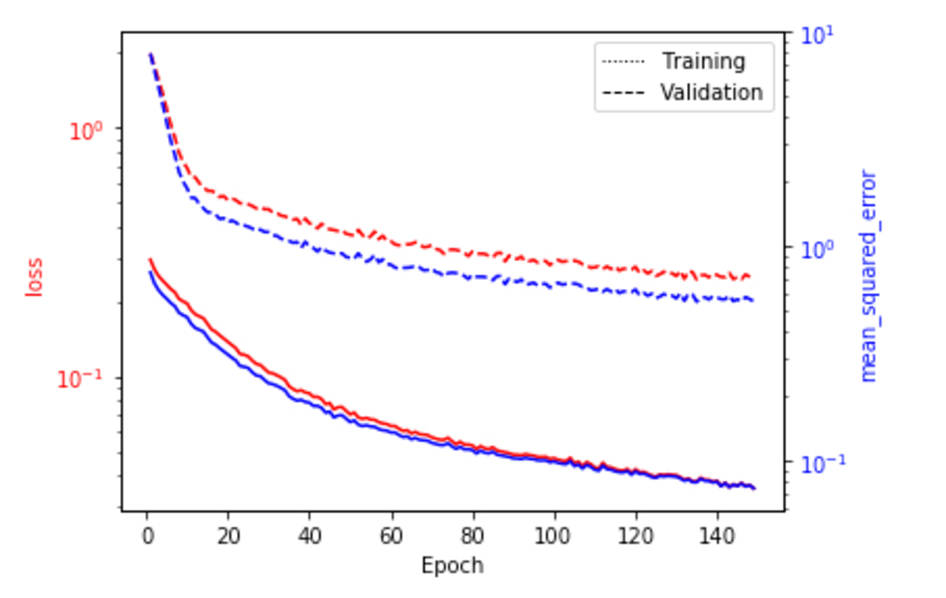
\includegraphics[width=0.8\textwidth]{log_lum_4_layer_2D_history.pdf}
				\caption{Loss history of the training of the 4 layer, 2D and log valued model.  Note that training data is actually the solid line not what the legend says.}
				\label{fig:log_lum_4_layer_2D_history}
			\end{figure}

			\begin{figure}[H]
				\centering
				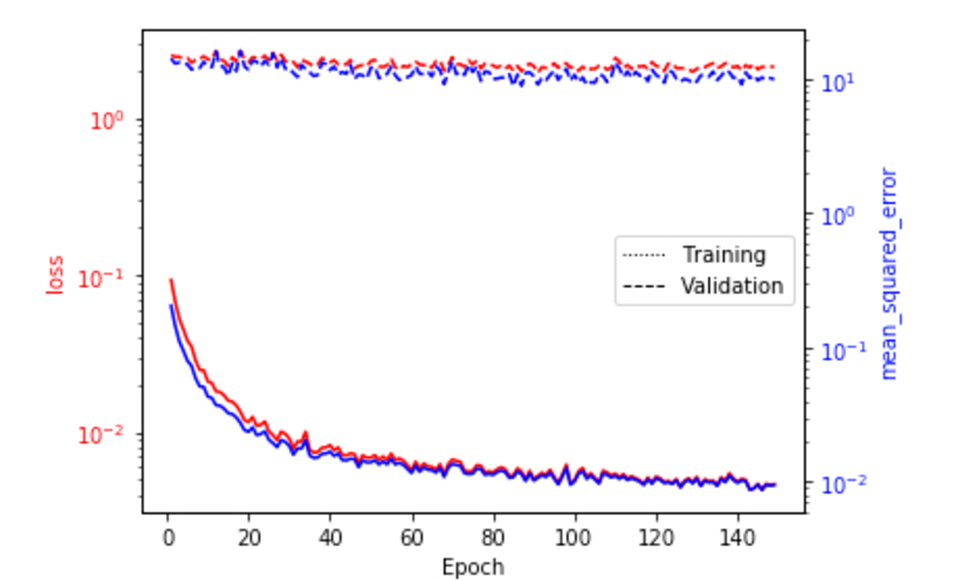
\includegraphics[width=0.8\textwidth]{log_lum_4_layer_history.pdf}
				\caption{Loss history of the training of the 4 layer and log valued model.  Note that training data is actually the solid line not what the legend says.}
				\label{fig:log_lum_4_layer_history}
			\end{figure}

			I don't have models in both 2D and 3D for testing against \(\phi\) or \(\phi L\) to see how they differ between the dimensions.

		\subsection{What is actually working?} \label{sec:wiaw}

			\begin{figure}[H]
				\centering
				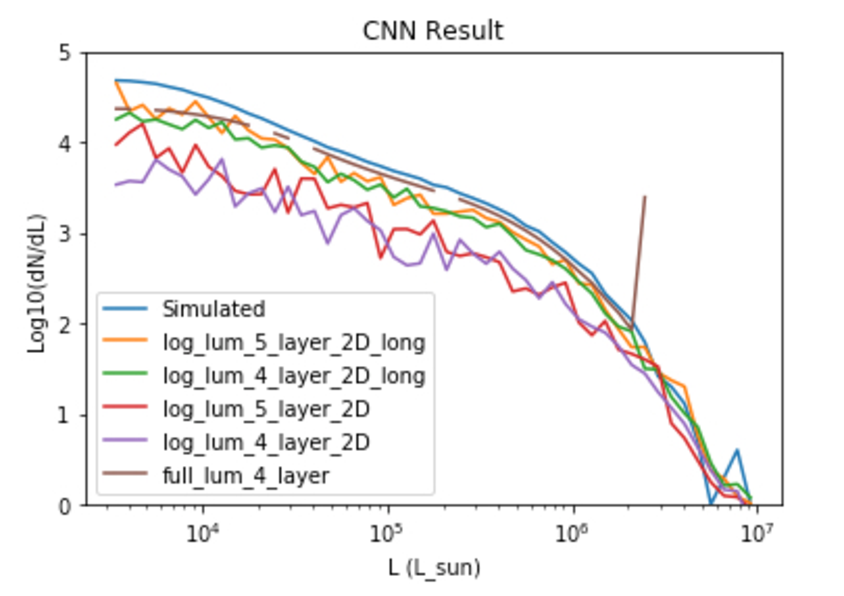
\includegraphics[width=0.8\textwidth]{compare_models.pdf}
				\caption{Comparison of the output from a few different models.}
				\label{fig:compare_models}
			\end{figure}

			Now lets try to figure out what is working and what we should be continuing on with.  \cref{fig:compare_models} shows the output from a few different models for a single map.  Note that not every model was trained on log data, but it is presented in log space now.  A few things become apparent by looking at the curves.  First is that the longer training models did better then the less trained models.  This is seen comparing the 4 and 5 layer 2D log data v.s. the long version of those.  \dnp{Who could have guessed this?}  The next thing to notice is that the 4 layer network trained on the full luminosity function isn't bad.  I would have expected this to be awful.  The range of values it needs to get is very large, but it was one of the best trained models.  It does have some holes in it's range which we saw earlier for a similar model in \cref{fig:CNN_4_layer}.  I don't know why those things are appearing, but they do.  \dnp{Maybe more training will help?}  

			More models were tested then what is in the figure, but the best were shown.

			In \cref{fig:compare_models_ratio} we can look at the ratio of model output to expected output as a function of \(L\).  In this figure we see that the 4 layer full luminosity function model is best at times with the 5 layer 2D log value one behind that and the 4 layer version of the previous model slightly worse off.

			\begin{figure}[H]
				\centering
				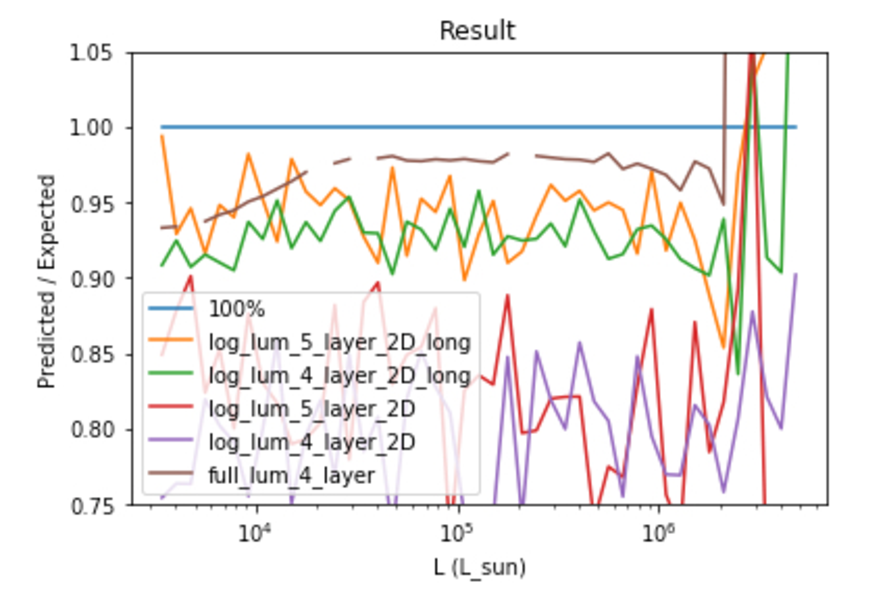
\includegraphics[width=0.8\textwidth]{compare_models_ratio.pdf}
				\caption{Comparison of the ratio of output to expected value from a few different models.}
				\label{fig:compare_models_ratio}
			\end{figure}

			Again it is useful to look at the training history.  When comparing the 4 layer and 5 layer histories in \cref{fig:log_lum_4_layer_2D_model_long_history,fig:log_lum_5_layer_2D_model_long_history} we see that there is a big gap between the training in validation for 4 layers, but not for 5 layers.  It might be that the network isn't big enough with 4 layers to learn as fast as it can.  The 5 layer network learns very nicely and doesn't appear to be leveling out yet when the training ended.  I don't know how, but somehow training in 3D gave a terrible history which can be seen in \cref{fig:full_lum_4_layer_model_history}.  The training and validation loss data are mostly the same after about 40 epochs, but it oscillates which is weird.  The mse error improves for some reason even though it isn't being trained on that and the loss isn't really improving.

			\begin{figure}[H]
				\centering
				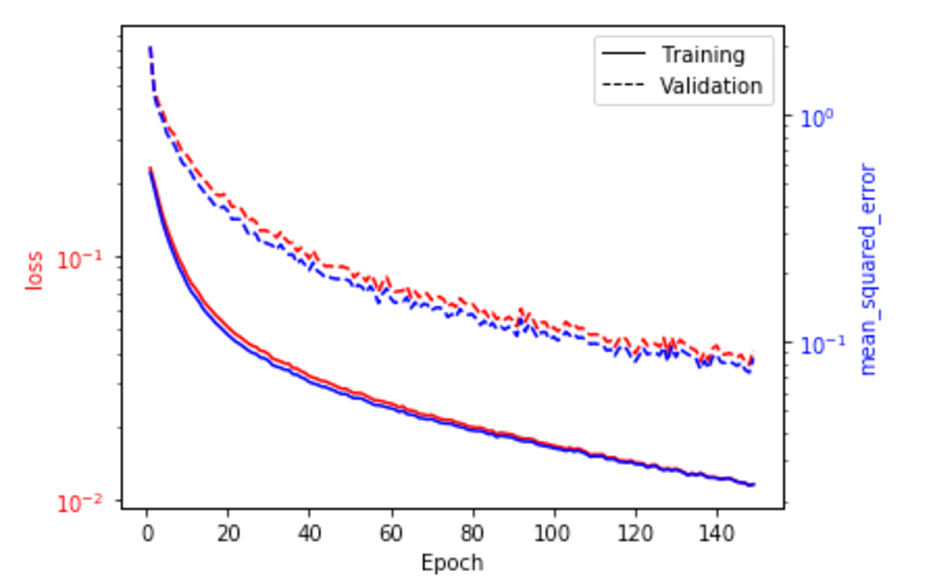
\includegraphics[width=0.8\textwidth]{log_lum_4_layer_2D_model_long_history.pdf}
				\caption{Loss history of the training of the 4 layer 2D log valued model.}
				\label{fig:log_lum_4_layer_2D_model_long_history}
			\end{figure}

			\begin{figure}[H]
				\centering
				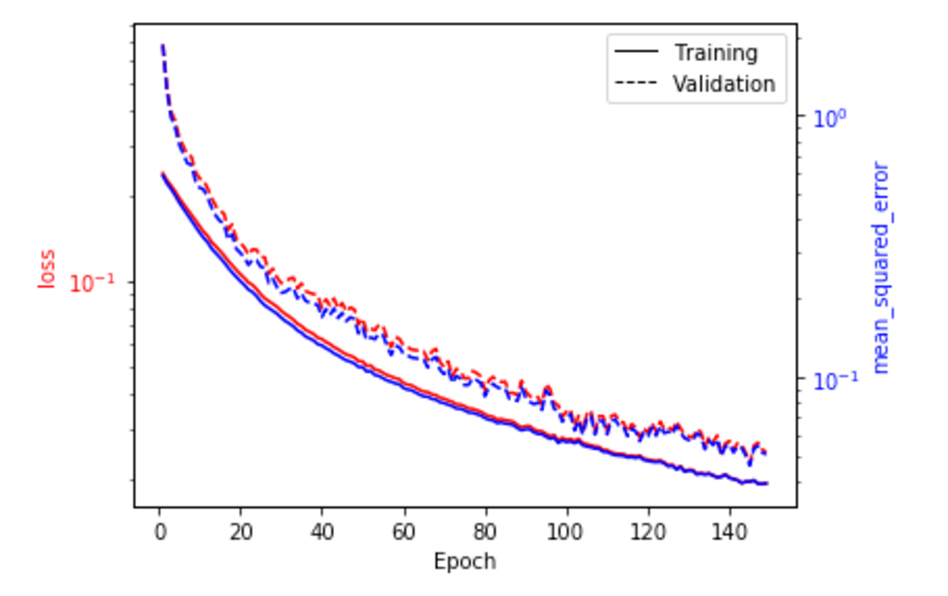
\includegraphics[width=0.8\textwidth]{log_lum_5_layer_2D_model_long_history.pdf}
				\caption{Loss history of the training of the 5 layer 2D log valued model.}
				\label{fig:log_lum_5_layer_2D_model_long_history}
			\end{figure}

			\begin{figure}[H]
				\centering
				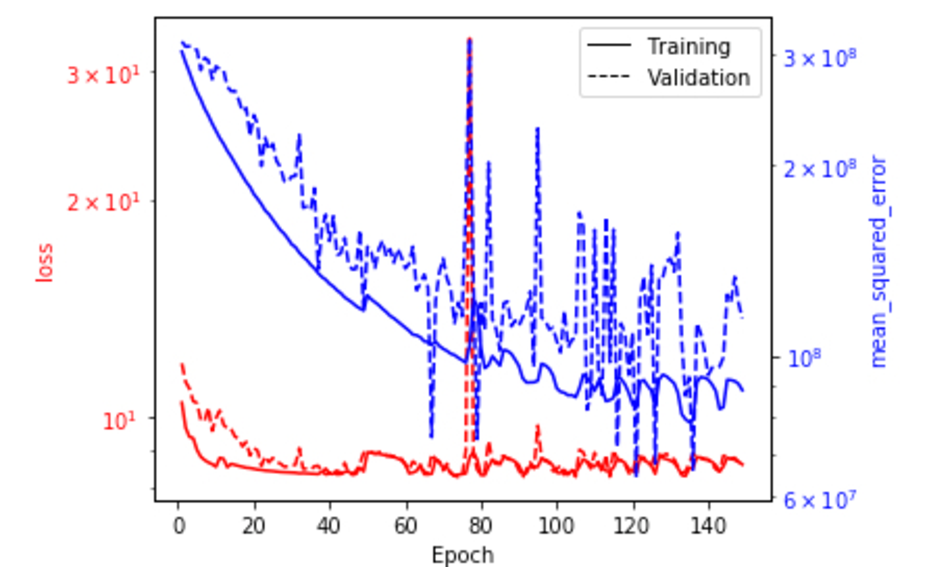
\includegraphics[width=0.8\textwidth]{full_lum_4_layer_model_history.pdf}
				\caption{Loss history of the training of the 4 layer full valued model.}
				\label{fig:full_lum_4_layer_model_history}
			\end{figure}

	\section{Training and Testing Regime} \label{sec:tat}
		Once we determine what architectures we are using we must determine what we want to train and test our networks on.  As of right now we have 3 luminosity models with uncertainty on parameters.  We don't have any noise or uncertainty due to astrophysics, cosmology or the detector yet.  That will need to be put into the map making process.

		I think first we will decide what architectures to train with.  We can pick a few like log 4 layer 2D and log 4 layer (which is 3D) and full 5 layer as an example.  After we pick the architectures we need to determine what we are training on.  I believe we should train a network for each architecture on the following
		\begin{enumerate}
			\item All base luminosity models (Just a single model at a time)

			\item All luminosity models with random values used for parameters in each map (Just a single model at a time)

			\item Combined models with base parameters

			\item Combined models with random parameters

			\item All previous scenarios with noise added
		\end{enumerate}
		From this we need to determine which model works best in each scenario that matters.  My naive guess would be models trained on noise will be better with noise and models without noise would be better for future experiments with less noise.


	\section{Things to do for Dan in no particular order}
		\begin{enumerate}
			\item Figure out what a good frequency bin size is

			\item \sout{Make maps and luminosity functions. Have done this for some maps and have the ability to do this for more.}

			\item \sout{Add in different halo luminosity relations to llm}

			\item \sout{Do some test runs with something basic}

			\item \sout{Make an actual CNN and try training it for an extended period of time}

			\item \sout{Get GPUs working correctly}

			\item \sout{Train on actual luminosity function instead of log(luminosity function). Doesn't give the best results.  See Section \ref{sec:4directValue} (and this was done on \(N\) not \(\phi\)).}

			\item \sout{Get CNN to record loss and metric as it trains}

			\item \sout{Make lots of maps on MARCC to train with.  This will happen soon.}

			\item \sout{Use validation data to see that the model is actually learning and not memorizing.}

			\item Figure out what architecture we actually want to use and start the actual training and testing
		\end{enumerate}


	
% \bibliography{draft}
\end{document}